% "{'classe':('PSI'),'chapitre':'slci_pi','type':('td'),'titre':'La robotique au service du handicap', 'source':'Centrale Supélec - PSI 2010','comp':('C1-02','C2-04'),'corrige':False}"
%\setchapterimage{bandeau}
\chapter*{TD \arabic{cptTD} \\ 
La robotique au service du handicap -- 
\ifprof Corrigé \else Sujet \fi}
\addcontentsline{toc}{section}{TD \arabic{cptTD} :
La robotique au service du handicap -- 
\ifprof Corrigé \else Sujet \fi}

\iflivret \stepcounter{cptTD} \else
\ifprof  \stepcounter{cptTD} \else \fi
\fi

\setcounter{question}{0}
\marginnote{Centrale Supélec -- PSI 2010.}
\marginnote[1cm]{
\UPSTIcompetence[2]{C1-02}
\UPSTIcompetence[2]{C2-04}}

\begin{marginfigure} [4cm]
\centering
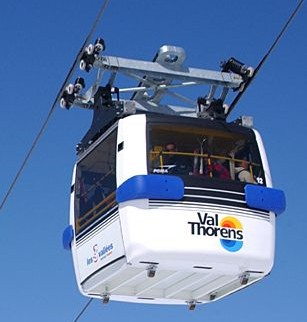
\includegraphics[width=.8\linewidth]{fig_00}
\end{marginfigure}



\subsection*{Présentation}
On s'intéresse à la conception de la loi de commande d'un des moteurs d'une orthèse d'épaule permettant d'améliorer le rétablissement de patients en cours de rééducation. 

\begin{obj}
\begin{itemize}
\item Temps de réponse à 5\% pour un échelon de consigne de couple : $t\leq \SI{2}{ms}$.
\item Erreur statique pour un couple de référence constant $C_{\text{ref 0}}$ : $|\varepsilon_0 |\leq 0,05 C_{\text{ref 0}}$.
\item Couple maximal fourni sur l’axe de l’articulation $C_{\text{max}} = \SI{50}{Nm}$.
\end{itemize}
\end{obj}

En pratique, le couple délivré par le moteur ne peut être mesuré directement, c’est pourquoi la grandeur
asservie est le courant moteur. L’objet, dans cette phase de l’étude, est alors de déterminer une loi de
commande pour la boucle d’asservissement et de valider les performances vis-à-vis du cahier des charges
partiel.

On donne partiellement le schéma-blocs de la commande. 

\begin{center}
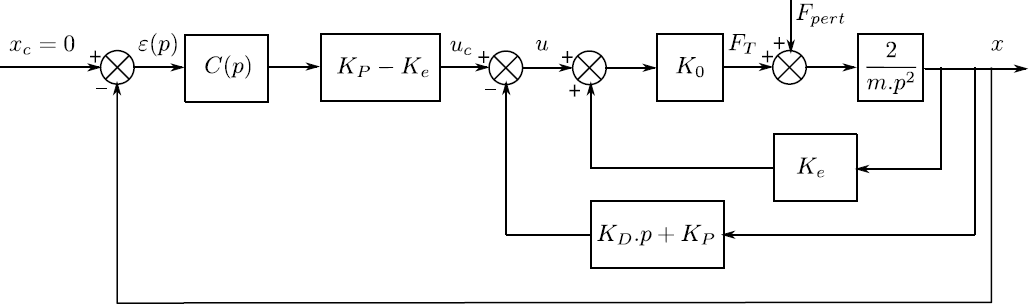
\includegraphics[width=1.0\linewidth]{fig_02}
\end{center}

Le correcteur choisi est de type proportionnel-intégral (P.I.) de fonction de transfert : $C(p)=K\left(1+\dfrac{1}{T_ip}\right)$. On adopte sans aucune justification que $T_i=\SI{0,3}{ms}$. 
Le diagramme de Bode de la fonction de transfert en boucle ouverte non corrigée 
\footnotesize
$$
H(p)=\dfrac{
0,0326 p \left( 1+\dfrac{2\times 0,08}{463}p+\dfrac{p^2}{463^2}\right)}
{
\left(1+\dfrac{p}{122} \right)
\left( 1+\dfrac{2\times 0,09}{464}p+\dfrac{p^2}{464^2}\right)
\left(1+\dfrac{p}{10^3} \right)
\left(1+\dfrac{p}{10^4} \right)
}
$$
\normalsize
est donné en fin de document. $i_{\text{mes}}(t)$ est la mesure du courant du moteur et $u(t)$ la tension d’alimentation. Ce tracé pourra être utilisé sans aucune justification.


\subsection*{Syntèse du régulateur PI de la boucle de courant}
\question{Compléter le diagramme de Bode par le tracé des diagrammes asymptotiques de la fonction $H(p)$.}
\ifprof
\begin{corrige}
\end{corrige}
\else
\fi

\question{En adoptant $K = 1$, tracer le diagramme de Bode
(module et phase) de $C(p)$ : diagrammes asymptotiques et allures des tracés réels avec les valeurs prises aux points caractéristiques.}
\ifprof
\begin{corrige}
\end{corrige}
\else
\fi

\question{En déduire les tracés asymptotiques et les allures des tracés réels du diagramme de Bode de la fonction de transfert en boucle ouverte corrigée (on différenciera les tracés par des
couleurs différentes). Déterminer, sans calcul supplémentaire, la pulsation $\omega_1$ telle que la phase de la fonction
de transfert en boucle ouverte est égale à \SI{-135}{\degres} et la valeur numérique du gain statique.
}
\ifprof
\begin{corrige}
\end{corrige}
\else
\fi


\question{Déterminer alors la valeur du gain $K$ permettant d’assurer une marge de phase de 45\degres.}
\ifprof
\begin{corrige}
\end{corrige}
\else
\fi

On considère maintenant le système corrigé avec le correcteur $C(p)$ qui vient d’être déterminé.


\question{Déterminer un ordre de grandeur de la marge de gain obtenue et conclure sur la stabilité du système en
boucle fermée.}
\ifprof
\begin{corrige}
\end{corrige}
\else
\fi


\question{Déterminer l'écart statique $\Delta i_0 = \lim\limits_{t\to +\infty} \left(i_c(t)-i_{\text{mes}}(t)\right)$ en boucle fermée en réponse à un échelon de consigne $i_c(t) = I_0\Gamma(t)$ d’amplitude $I_0$ et l’exprimer sous la forme $\Delta i_0 =  kI_0$ en précisant la valeur numérique de $k$.
}
\ifprof
\begin{corrige}
\end{corrige}
\else
\fi

\begin{marginfigure}
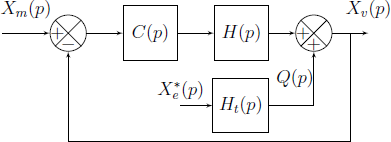
\includegraphics[width=1.0\linewidth]{fig_03}
\end{marginfigure}

La figure suivante représente la structure de l’actionneur (la boucle de courant du moteur étant fermée) : $i_c$ et $i$
sont respectivement la consigne et le courant moteur, $C_{\text{ref}}$ est le couple de référence souhaité, $C_a$ est le couple
appliqué par l’actionneur sur l’axe de l’articulation et $G_{ic}$ est un gain pur correspondant à la relation entre le
courant et le couple $C_a$. On suppose pour toute cette question que le couple de référence $C_{\text{ref}} (t)$ est constant
d’amplitude $C_{\text{ref}} = C_{\text{ref0}}$.



\question{Exprimer $G_{ic}$ en fonction de $K_c$ et de~$N$.
}
\ifprof
\begin{corrige}
\end{corrige}
\else
\fi


\question{
En supposant qu’en régime permanent l’erreur statique de la boucle d’asservissement de courant est nulle
$\Delta i_0= 0$, donner la valeur du gain $G_0$ permettant d’assurer l’égalité des couples de référence $C_{\text{ref0}}$ et appliqué $C_a$.}
\ifprof
\begin{corrige}
\end{corrige}
\else
\fi

\question{
En remarquant que le gain statique du capteur de courant est de 1, montrer, en utilisant les résultats des questions précédentes, qu’en régime permanent l’erreur $\Delta C= C_{\text{ref}} -C_a$
entre le couple de référence et le couple moteur exprimé sur l’axe de l’articulation est $\Delta C= k_1C_{\text{ref0}}$. Déterminer $k_1$ en fonction de $k$.}
\ifprof
\begin{corrige}
\end{corrige}
\else
\fi


\question{Vérifier alors si les différentes exigences du cahier des charges de l’actionneur sont validées.
}
\ifprof
\begin{corrige}
\end{corrige}
\else
\fi

On admettra sans aucune justification que la pulsation de coupure à $\SI{0}{dB}$ et le temps de réponse sont liés par la relation approximative $\omega_cTr \simeq 3$.


\ifcolle
\else
\marginnote{
\begin{solution}
\begin{enumerate}
\item .
\item .
\item $\omega_1 = \SI{3300}{rad.s^{-1}}$ et gain statique de 1,4.
\item $K = 0,7$.
\item Marge de gain infinie, marge de phase positive.
\item $\Delta i_0 = \dfrac{1}{1+K_{bo}}I_0$.
\item $G_{\text{ic}} = K_c N$.
\item $G_0 = \dfrac{1}{G_{\text{ic}}}$.
\item $k_1 = k$.
\item OK.
\end{enumerate}
\end{solution}}
\normalsize
\fi

\ifprof
\else
\begin{marginfigure}
\centering

\includegraphics[width=3cm]{Cy_03_01_TD_PI_06_Robotique_qr}
\end{marginfigure}
\fi



\begin{center}
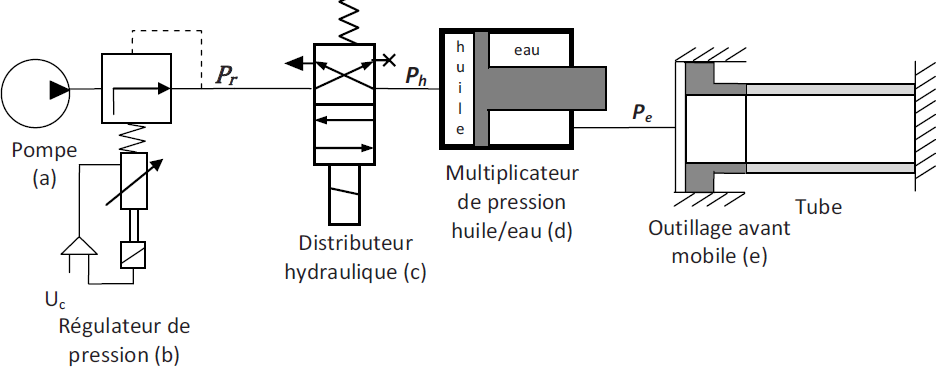
\includegraphics[width=1.0\linewidth]{fig_01}
\end{center}
